\documentclass[11pt]{article}

\usepackage[margin=1in]{geometry}
\usepackage{lmodern}
\usepackage[T1]{fontenc}
\usepackage{microtype}
\usepackage{amsmath, amssymb, amsthm, mathtools, bm}
\usepackage{booktabs}
\usepackage{enumitem}
\usepackage{xcolor}
\usepackage{tikz}
\usepackage{float}
\usepackage{algorithm}
\usepackage{algpseudocode}
\usepackage[colorlinks=true, linkcolor=blue!50!black, citecolor=blue!50!black,
            urlcolor=blue!50!black]{hyperref}

\newtheorem{proposition}{Proposition}
\theoremstyle{remark}
\newtheorem{remark}{Remark}

\newcommand{\x}{\bm{x}}
\newcommand{\y}{\bm{y}}
\newcommand{\uu}{\bm{u}}
\newcommand{\vv}{\bm{v}}
\newcommand{\eps}{\bm{\varepsilon}}
\newcommand{\zz}{\bm{z}}
\newcommand{\nn}{\bm{n}}
\newcommand{\cc}{\bm{c}}
\newcommand{\E}{\mathbb{E}}
\newcommand{\R}{\mathbb{R}}
\newcommand{\N}{\mathcal{N}}
\newcommand{\Id}{\bm{I}}
\newcommand{\Op}{\bm{E}}
\newcommand{\grad}{\nabla}
\newcommand{\PMI}{\operatorname{PMI}}
\newcommand{\ssb}{\sigma_{\mathrm{sb}}}
\newcommand{\code}[1]{\texttt{#1}}
\newcommand{\D}{D_\theta}
\newcommand{\Dz}{D_{\varnothing}}
\newcommand{\Dg}{D_{\x_1}}
\newcommand{\Dy}{D_{\y}}
\newcommand{\Dgy}{D_{\x_1,\y}}

\title{ImMAP: guided posterior ascent,\\[2pt]
       \large with and without a bridge}
\author{ImMAP project notes}
\date{November 2026}

\begin{document}
\maketitle

\begin{abstract}
We want the MAP estimate of a target image $\x_0$ given the side information available: a guide
image $\x_1$ (a paired scan, typically of another contrast), a measurement $\y$, or both.
Revealing the side information one variable at a time splits the log-posterior exactly into
the target prior plus one likelihood term per variable. The split survives Gaussian smoothing,
and by Tweedie's formula the gradient of each term is a difference of conditional expectations.
One annealed ascent step therefore serves every conditioning set; ImMAP2 is a case study. A
denoiser must be evaluated at every smoothing level, including very large ones, and that is
where a bridge helps. It feeds the network a bridge sample that carries the same information as
a very noisy target but stays bounded. I$^2$SB is the ascent run through this bridge
preconditioner, and each line of its sampler is a reparameterised line of the ascent.
\end{abstract}

\paragraph{Setting.} Real vectors in $\R^n$; the complex case is identical with Wirtinger
gradients. Pairs $(\x_0,\x_1)$ have a joint law. The measurement is $\y = \Op\x_0 + \nn$, with
$\nn\sim\N(\bm0,\sigma_n^2\Id)$ independent of $(\x_0,\x_1)$, so $\y$ and $\x_1$ are conditionally
independent given $\x_0$. The noisy target is $\uu = \x_0 + \sigma\eps$, with
$\eps\sim\N(\bm0,\Id)$ independent of everything else. For a set $\cc\subseteq\{\x_1,\y\}$ of
conditioning variables,
\[
  D_{\cc}(\uu,\sigma) \coloneqq \E[\x_0\mid\uu,\cc]\quad\text{at noise level } \sigma .
\]

%=============================================================================================
\section{The objective}
%=============================================================================================

Given side information $\cc$, the goal is
\begin{equation}
  \hat\x_0 = \arg\max_{\x_0}\ \log p(\x_0\mid\cc),
  \qquad \cc\in\big\{\varnothing,\ \{\x_1\},\ \{\y\},\ \{\x_1,\y\}\big\}.
  \label{eq:map}
\end{equation}
We always condition on every independent source of information available. A variable that is a
function of others adds nothing. For example, the zero-filled image $\Op^H\y$ is a function of
$\y$, so conditioning on it as well as on $\y$ is conditioning on $\y$. A guide scan is not, so
$p(\x_0\mid\x_1,\y)\ne p(\x_0\mid\y)$ in general.

%=============================================================================================
\section{Decomposing along a chain}
%=============================================================================================

Reveal the variables of $\cc$ one at a time, in some order. With two variables, guide first:
\begin{align}
  \log p(\x_0\mid\x_1,\y)
  &= \log p(\x_0)
   + \underbrace{\log\frac{p(\x_0\mid\x_1)}{p(\x_0)}}_{\PMI(\x_0;\,\x_1)}
   + \underbrace{\log\frac{p(\x_0\mid\x_1,\y)}{p(\x_0\mid\x_1)}}_{\PMI(\x_0;\,\y\mid\x_1)}
  \label{eq:chain}\\
  &= \log p(\x_0) + \log p(\x_1\mid\x_0) + \log p(\y\mid\x_0) + \mathrm{const}.
  \label{eq:likelihoods}
\end{align}
\eqref{eq:chain} is an identity, because the ratios telescope. Each pointwise mutual
information (PMI) term measures how much the newly revealed variable says about $\x_0$, given
what was revealed before. In \eqref{eq:likelihoods} each becomes a likelihood:
\begin{itemize}[leftmargin=1.5em, itemsep=1pt]
  \item by Bayes, $\PMI(\x_0;\bm a\mid\bm b) = \log p(\bm a\mid\x_0,\bm b) - \log p(\bm a\mid\bm
        b)$, and the last term does not depend on $\x_0$;
  \item by conditional independence, $p(\y\mid\x_0,\x_1) = p(\y\mid\x_0)$.
\end{itemize}
So the objective is
\begin{center}
  \emph{target prior} $+$ \emph{guide likelihood} $+$ \emph{measurement likelihood},
\end{center}
whichever order the variables are revealed in, and dropping a variable drops its term. With one
variable the chain has one step; with none, \eqref{eq:map} is the prior alone.

The order does not change the objective. It changes the intermediate conditional expectations
that appear below, that is, which estimators the gradient is assembled from. Guide-first uses
$\Dz,\Dg,\Dgy$; measurement-first uses $\Dz,\Dy,\Dgy$.

%=============================================================================================
\section{Smoothing, and the gradient}
%=============================================================================================

As in ImMAP~\cite{ks2021}, we ascend a Gaussian smoothing of the objective while lowering the
smoothing. Let
\[
  J_\sigma(\uu) \coloneqq \log p_\sigma(\uu\mid\cc),\qquad
  p_\sigma(\uu\mid\cc) = \int\N(\uu;\x,\sigma^2\Id)\,p(\x\mid\cc)\,d\x .
\]
So $J_\sigma$ is the log-density of the noisy target given $\cc$, and $J_\sigma\to\log
p(\cdot\mid\cc)$ as $\sigma\to0$.

\begin{proposition}[The chain survives smoothing; each term is a difference of expectations]
\label{prop:grad}
Along the chain $\varnothing\subset\cc_1\subset\dots\subset\cc_K = \cc$,
\begin{equation}
  J_\sigma(\uu) = \log p_\sigma(\uu)
  + \sum_{k=1}^K \log\frac{p_\sigma(\uu\mid\cc_k)}{p_\sigma(\uu\mid\cc_{k-1})},
  \qquad
  \sigma^2\grad J_\sigma(\uu) = \underbrace{\Dz + \sum_{k=1}^K\big(D_{\cc_k}-D_{\cc_{k-1}}\big)}
  _{=\ D_{\cc}(\uu,\sigma)} -\ \uu ,
  \label{eq:grad}
\end{equation}
and each ratio is the PMI between the \emph{noisy} target $\uu$ and the $k$-th variable.
\end{proposition}
\begin{proof}
The telescoping is the same as in \eqref{eq:chain}, with $\uu$ in place of $\x_0$. Bayes applies
to $(\uu,\cc_k)$ because $\eps$ is independent of the side information. Tweedie's formula,
$\sigma^2\grad\log p_\sigma(\uu\mid\cc_k) = D_{\cc_k}(\uu,\sigma) - \uu$, holds for any such
$\cc_k$ (differentiate the convolution under the integral). Apply it to every term; the
$-\uu$'s cancel inside each ratio.
\end{proof}

\emph{What a variable contributes to the gradient is how far revealing it moves the conditional
expectation}, $D_{\cc_k} - D_{\cc_{k-1}}$. It vanishes when the variable is uninformative given
the others. Summed, the chain gives back $D_{\cc}$, so an estimator of $D_{\cc}$ itself needs
nothing else. The decomposition earns its keep when $D_{\cc}$ is \emph{not} directly
available. Then one estimates a less-conditioned expectation and adds the last increment
separately. That is exactly what a data-consistency step does,
\[
  \Dgy = \Dg + \underbrace{(\Dgy - \Dg)}_{\text{measurement term}},
\]
with the increment estimated from the measurement model (Section~\ref{sec:estimators}).

The smoothed terms are not the unsmoothed likelihoods at a noisy image. The measurement term,
for instance, involves $p(\y\mid\uu,\x_1) = \int p(\y\mid\x)\,p(\x\mid\uu,\x_1)\,d\x$: the
likelihood averaged over the targets the noisy state still allows. It is weak at large $\sigma$
and sharpens to $p(\y\mid\x_0)$ as $\sigma\to0$.

%=============================================================================================
\section{The ascent}\label{sec:ascent}
%=============================================================================================

\paragraph{The step.} Gradient ascent on $J_\sigma$ with step size $h\sigma^2$ is, by
\eqref{eq:grad},
\begin{equation}
  \boxed{\;\uu^+ = \uu + h\sigma^2\grad J_\sigma(\uu) = (1-h)\,\uu + h\,\vv,
  \qquad \vv = D_{\cc}(\uu,\sigma).\;}
  \label{eq:step}
\end{equation}
Tweedie's second-order identity gives $-\grad^2 J_\sigma = (\sigma^2\Id -
\operatorname{Cov}[\x_0\mid\uu,\cc])/\sigma^4\preceq\sigma^{-2}\Id$. So every $h\in(0,2)$
increases $J_\sigma$, by the descent lemma, whatever $\cc$ is.

\paragraph{The continuation.} After each step, fresh noise is injected so that the iterate is
again a noisy target, at the next, smaller level $\sigma' = r\sigma$. An exact step leaves noise
$(1-h)\sigma$, so the injection is
\begin{equation}
  \gamma^2 = \sigma'^2 - (1-h)^2\sigma^2,
  \qquad\text{which needs } |1-h|\le r .
  \label{eq:inject}
\end{equation}
There are two ways to set $r$:
\begin{itemize}[leftmargin=1.5em, itemsep=1pt]
  \item ImMAP parameterises the contraction as $r = 1-\beta h$ with $\beta\in(0,1]$, which gives
        $\gamma = \sigma\sqrt{(1-\beta h)^2-(1-h)^2}$;
  \item a fixed ladder $\sigma_N>\dots>\sigma_0=0$ sets $r_k = \sigma_{k-1}/\sigma_k$ and
        leaves $h_k\in[1-r_k,1]$ free.
\end{itemize}

\begin{algorithm}[H]
\caption{Annealed posterior ascent for $\max_{\x_0}\log p(\x_0\mid\cc)$}
\label{alg:ascent}
\begin{algorithmic}[1]
\Require an estimator of $D_{\cc}$, direct or assembled along a chain \eqref{eq:grad}
\Require a start $\uu$ at level $\sigma$ ($\sigma=\infty$ allowed); a rule for $h$, $r$ with
         $|1-h|\le r$; $\sigma_{\min}$
\While{$\sigma>\sigma_{\min}$}
  \State $\vv \gets D_{\cc}(\uu,\sigma)$
         \Comment{$=\uu + \sigma^2\grad J_\sigma(\uu)$}
  \State choose $h$ and $r$
  \State $\uu \gets (1-h)\,\uu + h\,\vv + \sigma\sqrt{r^2-(1-h)^2}\;\zz$, \ $\zz\sim\N(\bm0,\Id)$
         \Comment{\eqref{eq:step}, \eqref{eq:inject}}
  \State $\sigma \gets r\sigma$
\EndWhile
\State \Return $\vv$
\end{algorithmic}
\end{algorithm}

\noindent Three step sizes are worth naming:
\begin{itemize}[leftmargin=1.5em, itemsep=1pt]
  \item $h = 1-r^2$ removes the variance $\sigma^2-\sigma'^2$ and injects
        $\gamma^2 = \sigma'^2(1-r^2)$. This is the VE ancestral sampler~\cite{song2021}
        ($\beta = 1/(1+r)$).
  \item $h = 1-r$ injects nothing: the deterministic continuation toward the MAP estimate, and the
        Euler step of the probability-flow ODE ($\beta=1$).
  \item $h=1$ jumps to the estimate and re-noises it: SDEdit-style restarts~\cite{meng2022}.
\end{itemize}
Any $\beta<1$ re-injects noise, so the ascent then returns (approximately) a posterior sample
rather than the MAP estimate.

\paragraph{The start.} At $\sigma=\infty$, $r=0$ forces $h=1$. The first step returns
$D_{\cc}(\cdot,\infty) = \E[\x_0\mid\cc]$, whatever $\uu$ is, and re-noises it: the ascent
warm-starts itself from the posterior mean. An end-to-end reconstruction network (TGVN, LGGS)
that regresses $\E[\x_0\mid\y,\x_1]$ in one shot is exactly that first step, without the rest.

%=============================================================================================
\section{Estimating the expectations}\label{sec:estimators}
%=============================================================================================

The algorithm consumes $D_{\cc}$ and is indifferent to its source:
\begin{itemize}[leftmargin=1.5em, itemsep=2pt]
  \item $\Dz$: a target-only denoiser, trained with the squared loss on $(\uu,\x_0)$.
  \item $\Dg$: a guide-conditioned denoiser. Section~\ref{sec:bridge} trains it on bridge
        samples.
  \item $\Dgy$, learned: a regressor that also sees $(\y,\Op)$ and the guide (SB-TGVN,
        BridgeLGGS).
  \item $\Dgy$ (or $\Dy$) from $\Dg$ (or $\Dz$) by a \textbf{data step}. Approximate the
        posterior given $\uu$ and the other variables by $\N(D,\varsigma^2\Id)$ around the
        estimator's output $D$. With the Gaussian likelihood, the posterior mean given $\y$ too
        is the proximal point
        \begin{equation}
          (\Op^H\Op + \lambda\Id)^{-1}(\Op^H\y + \lambda D),\qquad
          \lambda = \sigma_n^2/\varsigma^2,
          \label{eq:prox}
        \end{equation}
        solved by CG warm-started at $D$. The posterior variance is at most $\sigma^2$ on
        average ($\E\|\x_0 - D\|^2 = \mathrm{mmse}(\sigma)\le n\sigma^2$). So the principled
        weight follows the noise level, $\lambda(\sigma) = \sigma_n^2/(c\sigma^2)$ with
        $c\le1$.
\end{itemize}

%=============================================================================================
\section{Case study: ImMAP2}\label{sec:immap2}
%=============================================================================================

ImMAP2 (\code{diffusion/immap.py}) has no guide. It is Algorithm~\ref{alg:ascent} for the
unguided posterior.

\paragraph{The objective.} $\cc = \{\y\}$, and the chain $\varnothing\subset\{\y\}$ has one step:
\[
  \log p(\x_0\mid\y) = \log p(\x_0) + \log p(\y\mid\x_0) + \mathrm{const},
  \qquad
  \sigma^2\grad J_\sigma = \underbrace{(\Dz-\uu)}_{\text{prior pull}}
  + \underbrace{(\Dy-\Dz)}_{\text{measurement pull}} .
\]

\paragraph{The estimator.} Only $\Dz$ is learned. The measurement increment comes from the data
step \eqref{eq:prox} on $\Dz$, solved by CG to tolerance, with
\[
  \lambda_k = \lambda_0\,\sigma_n^2\,\frac{1+\sigma_k^2}{\sigma_k^2} .
\]
This is \eqref{eq:prox} with $\varsigma^2 = \sigma_k^2/(1+\sigma_k^2)$, the posterior variance
under a unit-variance Gaussian prior (the $\Pi$GDM rule). It follows the noise level.

\paragraph{The schedule.}
\begin{itemize}[leftmargin=1.5em, itemsep=1pt]
  \item \textbf{Self-paced ladder.} The level is re-estimated at every step from the residual,
        $\sigma_k^2 = \tfrac1n\|\Dz(\uu_k)-\uu_k\|^2$. For an MMSE denoiser this is slightly
        low on average: $\E\|\Dz-\uu\|^2 = n\sigma^2 - \mathrm{mmse}$.
  \item \textbf{Step size} $h_k = h_0k/(1+h_0(k-1))$ with $h_0 = 0.01$, growing toward $1$.
  \item \textbf{Injection} with $\beta = 0.05$, so $r = 1-\beta h$: a slow contraction that samples.
  \item \textbf{Start} $\mathrm{mean}(\Op^H\y) + \zz$ at $\sigma = 1$.
\end{itemize}
The implementation returns the final state $\uu$, not $\vv$.

%=============================================================================================
\section{Specialising to a bridge}\label{sec:bridge}
%=============================================================================================

\subsection{Why}

Algorithm~\ref{alg:ascent} needs the denoiser on the whole ladder, from very large (or
infinite) $\sigma$ down to $0$. At large $\sigma$ the input $\uu=\x_0+\sigma\eps$ is almost all
noise:
\begin{itemize}[leftmargin=1.5em, itemsep=1pt]
  \item its norm grows like $\sigma$;
  \item the network must return $\approx\E[\x_0\mid\cc]$ while discarding all of it.
\end{itemize}
Standard diffusion copes in two ways. It rescales the input, as EDM's
$c_{\mathrm{in}}(\sigma)\uu$ does~\cite{karras2022}. And it stops at a finite $\sigma_{\max}$,
paying for the mismatch between $\N(\bm0,\sigma_{\max}^2\Id)$ and $p_{\sigma_{\max}}$. ImMAP2
sidesteps the problem by starting low, at $\sigma=1$.

When the side information contains an image $\x_1$ close to $\x_0$, there is a better rescaling.
Fix $V>0$ and feed the network
\begin{equation}
  \x_t = \x_1 + c(\sigma)\,(\uu-\x_1),\qquad c(\sigma) = \frac{V}{\sigma^2+V} = 1-t,
  \qquad t = \frac{\sigma^2}{\sigma^2+V}\in[0,1].
  \label{eq:x}
\end{equation}

\begin{proposition}\label{prop:bridge}
If $\uu=\x_0+\sigma\eps$, then $\x_t = (1-t)\,\x_0 + t\,\x_1 + \ssb(t)\,\eps$ with
$\ssb(t)^2 = Vt(1-t)$. This is the Brownian-bridge marginal from $\x_0$ to $\x_1$, with
$V=4\tau^2$. Conversely,
\begin{equation}
  \uu = \frac{\x_t - t\,\x_1}{1-t},\qquad \sigma^2 = \frac{Vt}{1-t}.
  \label{eq:u}
\end{equation}
For fixed $\x_1$ and $t<1$ the map is a bijection. So $\E[\x_0\mid\x_t,\x_1] =
\E[\x_0\mid\uu,\x_1] = \Dg(\uu,\sigma)$: a regressor trained on bridge samples \emph{is} the
denoiser that Algorithm~\ref{alg:ascent} needs for $\cc=\{\x_1\}$.
\end{proposition}
\begin{proof}
Substitute: $\x_1 + (1-t)(\x_0+\sigma\eps-\x_1) = (1-t)\x_0 + t\x_1 + (1-t)\sigma\eps$, and
$(1-t)^2\sigma^2 = (1-t)^2\,Vt/(1-t) = Vt(1-t)$.
\end{proof}

The level $\sigma = \ssb/(1-t) = \sqrt V\sqrt{t/(1-t)}$ is a standard deviation. It diverges as
$t\to1$, although $\ssb\to0$, because $\ssb$ vanishes only like $\sqrt{1-t}$. (The finite
quantity $\ssb^2/(1-t)=Vt$ is the variance of the forward process before it is pinned at
$\x_1$.) So bridge time is the smoothing level, from $\sigma=0$ at $t=0$ to $\sigma=\infty$ at
$t=1$.

\paragraph{Why it may work better.} The bridge sample and the noisy target carry the same
information, but the bridge sample is the much better network input:
\begin{itemize}[leftmargin=1.5em, itemsep=1pt]
  \item \textbf{Bounded noise.} The noise the network sees, $c(\sigma)\sigma = \ssb(t)$, peaks
        at $\tau$ (at $t=\tfrac12$) and vanishes at both ends, while $\sigma$ runs from $0$ to
        $\infty$ (Figure~\ref{fig:ladder}).
  \item \textbf{Bounded signal, exact start.} The input stays near the segment from $\x_0$ to
        $\x_1$. At $\sigma=\infty$ it is exactly $\x_1$, a finite input the network is trained
        on. So the top of the ladder is $\sigma=\infty$ with no start mismatch, and the first
        step of Algorithm~\ref{alg:ascent} is the network's regression $\E[\x_0\mid\x_1]$.
  \item \textbf{A Wiener-filter preconditioner.} \eqref{eq:x} is $\E[\x_0\mid\uu]$ under the
        Gaussian prior $\x_0\sim\N(\x_1,V\Id)$. So the network is fed the linear-Gaussian
        denoiser's output, and an $\x_0$-predicting network learns only the correction. The
        better $\x_1$ predicts $\x_0$, the smaller that correction.
\end{itemize}
In theory nothing is gained: the optimal outputs are equal. In practice a finite network has to
fit the denoiser at every level, and the bridge removes the levels where that is hardest.

The bridge parameter $\tau$ encodes an assumed per-pixel spread $\sqrt V=2\tau$ of $\x_0-\x_1$.
It shapes the preconditioner and the ladder, but not the target: $\E[\x_0\mid\uu,\sigma,\x_1]$
does not depend on $V$. A guide of a different contrast fits the Gaussian assumption worse. That
makes the correction larger; it does not change what the network should learn.

\begin{figure}[H]
\centering
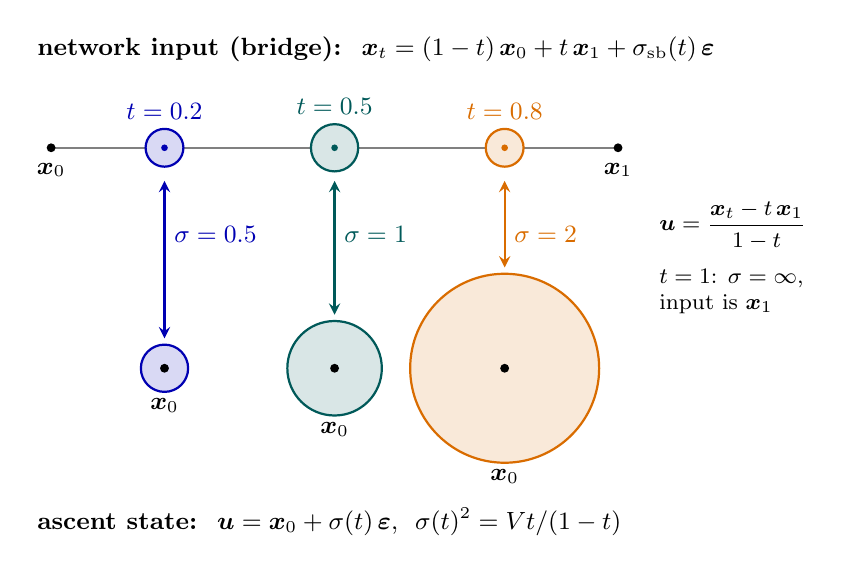
\begin{tikzpicture}[>=stealth, font=\small]
  \colorlet{ca}{blue!70!black}
  \colorlet{cb}{teal!70!black}
  \colorlet{cc}{orange!85!black}
  \node[anchor=west] at (-0.3, 1.25) {\textbf{network input (bridge):} \
        $\x_t = (1-t)\,\x_0 + t\,\x_1 + \ssb(t)\,\eps$};
  \draw[gray, thick] (0,0) -- (7.2,0);
  \fill (0,0) circle (1.6pt) node[below=2pt] {$\x_0$};
  \fill (7.2,0) circle (1.6pt) node[below=2pt] {$\x_1$};
  \foreach \t/\r/\c in {0.2/0.24/ca, 0.5/0.30/cb, 0.8/0.24/cc} {
    \fill[\c!15] (7.2*\t, 0) circle (\r);
    \draw[\c, thick] (7.2*\t, 0) circle (\r);
    \fill[\c] (7.2*\t, 0) circle (1.2pt);
    \node[\c, above] at (7.2*\t, \r) {$t = \t$};
  }
  \node[anchor=west] at (-0.3, -4.75) {\textbf{ascent state:} \
        $\uu = \x_0 + \sigma(t)\,\eps$, \ $\sigma(t)^2 = Vt/(1-t)$};
  \foreach \t/\r/\c/\s in {0.2/0.30/ca/0.5, 0.5/0.60/cb/1, 0.8/1.20/cc/2} {
    \fill[\c!15] (7.2*\t, -2.8) circle (\r);
    \draw[\c, thick] (7.2*\t, -2.8) circle (\r);
    \fill (7.2*\t, -2.8) circle (1.6pt);
    \node[below=-1pt] at (7.2*\t, -2.8 - \r) {$\x_0$};
    \draw[<->, \c, thick] (7.2*\t, -0.42) -- (7.2*\t, -2.8 + \r + 0.08);
  }
  \node[ca, right] at (1.44, -1.1) {$\sigma = 0.5$};
  \node[cb, right] at (3.60, -1.1) {$\sigma = 1$};
  \node[cc, right] at (5.76, -1.1) {$\sigma = 2$};
  \node[align=left, anchor=west, font=\footnotesize] at (7.6, -1.4)
        {$\uu = \dfrac{\x_t - t\,\x_1}{1-t}$\\[6pt]
         $t = 1$: $\sigma = \infty$,\\ input is $\x_1$};
\end{tikzpicture}
\caption{The same state in two coordinates. Bottom: the ascent state $\uu$, the target $\x_0$
plus noise $\sigma(t)$, which grows without bound toward $t=1$. Top: what the network is fed,
the bridge sample \eqref{eq:x}, whose noise $\ssb(t)$ stays below $\tau$ and vanishes at both
ends. The optimal outputs agree, $\E[\x_0\mid\x_t,\x_1] = \E[\x_0\mid\uu,\x_1]$. Radii drawn to
scale for $V=1$.}
\label{fig:ladder}
\end{figure}

\subsection{Training}

The bridge loss $\E\|\D(\x_t,t,\x_1)-\x_0\|^2$, with $t\sim\mathcal U[0,1]$, is conditional
denoising with the preconditioner \eqref{eq:x}. In EDM's vocabulary, only the design choices
differ from a standard conditional diffusion:

\begin{center}
\small
\begin{tabular}{@{}lll@{}}
\toprule
 & conditional VE diffusion & bridge \\
\midrule
ideal denoiser & $\E[\x_0\mid\uu,\sigma,\x_1]$ & the same \\
network input & $c_{\mathrm{in}}(\sigma)\,\uu$, e.g.\ $(\sigma^2+\sigma_{\mathrm{data}}^2)^{-1/2}\uu$
  & $\x_1 + c(\sigma)(\uu-\x_1)$ \\
training levels & e.g.\ log-normal $\sigma$ & $p(\sigma) = 2\sigma V/(\sigma^2+V)^2$ \\
top level & finite $\sigma_{\max}$, start $\N(\bm0,\sigma_{\max}^2\Id)$ & $\infty$, start $\x_1$ \\
sampling ladder & e.g.\ $\rho$-spaced in $\sigma$ & uniform in $t$ \\
\bottomrule
\end{tabular}
\end{center}

\noindent The identity needs a network that is given $\x_1$. Without \code{cond\_x1} (as in
I$^2$SB-Inversion) it learns $\E[\x_0\mid\x_t]$. That network reads $\x_1$ only through $\x_t$,
which works near $t=1$ but is not the conditional denoiser in general.

\paragraph{Relation to unconditional diffusion.} Since $\uu$ and $\x_1$ are independent given
$\x_0$, Bayes' rule splits the score, and Tweedie turns the split into denoisers:
\begin{equation}
  \E[\x_0\mid\uu,\x_1] = \E[\x_0\mid\uu] + \sigma^2\,\grad_{\uu}\log p_\sigma(\x_1\mid\uu).
  \label{eq:bayes}
\end{equation}
This is the guide's PMI increment of Proposition~\ref{prop:grad}, $\Dg-\Dz$. A bridge learns
it, where DPS~\cite{chung2023} approximates it through the denoiser's Jacobian. It follows that
a conditional-diffusion baseline on the same $\x_1$ (SR3/Palette style) is not an independent
method: same target, same sampler family. Any gap in results comes from the design choices in
the table above.

%=============================================================================================
\section{Case study: I\texorpdfstring{$^2$}{2}SB}\label{sec:i2sb}
%=============================================================================================

The source image $\x_1$ is the only side information; there is no measurement.

\paragraph{The objective.} $\cc = \{\x_1\}$, and the chain $\varnothing\subset\{\x_1\}$ has one
step:
\[
  \log p(\x_0\mid\x_1) = \log p(\x_0) + \log p(\x_1\mid\x_0) + \mathrm{const},
  \qquad
  \sigma^2\grad J_\sigma
  = \underbrace{\big(\Dz - \uu\big)}_{\text{prior pull}}
  + \underbrace{\big(\Dg - \Dz\big)}_{\text{what } \x_1 \text{ adds}}
  = \Dg - \uu .
\]
A target that is plausible on its own and consistent with this particular source. I$^2$SB never
splits the two pulls: its network estimates their sum, $\Dg$, directly.

\subsection{The ascent I\texorpdfstring{$^2$}{2}SB runs}

Take Algorithm~\ref{alg:ascent} with $\cc=\{\x_1\}$ and three settings:
\begin{itemize}[leftmargin=1.5em, itemsep=1pt]
  \item the ladder $\sigma_k=\sigma(t_k)$ on a grid $1=t_N>\dots>t_0=0$, so $\sigma_N=\infty$;
  \item the ancestral step $h_k = 1-r_k^2$, that is $\beta_k = 1/(1+r_k)$;
  \item the denoiser read through Proposition~\ref{prop:bridge},
        $\Dg(\uu,\sigma) = \D(\x_1 + c(\sigma)(\uu-\x_1),\,t(\sigma),\,\x_1)$.
\end{itemize}
Write $t=t_k$, $s=t_{k-1}$. By \eqref{eq:u}, $r^2 = \sigma_s^2/\sigma_t^2 = \frac{s(1-t)}{t(1-s)}$,
and the step is
\begin{equation}
  \uu_s = r^2\,\uu_t + (1-r^2)\,\vv + \sigma_s\sqrt{1-r^2}\;\zz,\qquad
  \vv = \Dg(\uu_t,\sigma_t).
  \label{eq:ustep}
\end{equation}
The step size is the variance removed, and the injection tops the leftover noise
$r^2\sigma_t = r\sigma_s$ back up to exactly $\sigma_s$. This is \code{debiased\_ascent} in
\code{sb/i2sb\_recon.py}.

\subsection{Line by line into I\texorpdfstring{$^2$}{2}SB}

Map every state to the network's coordinates with \eqref{eq:x}, $\x_t = (1-t)\,\uu_t + t\,\x_1$:

\begin{center}
\small
\begin{tabular}{@{}lll@{}}
\toprule
line & ascent in $\uu$ (Algorithm~\ref{alg:ascent}) & I$^2$SB in $\x$ \\
\midrule
start & $\sigma_N=\infty$, $\uu_N$ arbitrary & $\x_{t_N} = \x_1$ \\
denoise & $\vv = \Dg(\uu_t,\sigma_t)$ & $\hat\x_0 = \D(\x_t,t,\x_1)$ \\
step & $\uu_s = r^2\uu_t + (1-r^2)\vv + \sigma_s\sqrt{1-r^2}\,\zz$
  & $\x_s = \tfrac st\x_t + \big(1-\tfrac st\big)\hat\x_0 + \sqrt{V\tfrac{s(t-s)}{t}}\,\zz$ \\
return & $\uu_0 = \vv$ at $\sigma_0=0$ & $\x_0 = \hat\x_0$ at $t_0=0$ \\
\bottomrule
\end{tabular}
\end{center}

\begin{proposition}\label{prop:lines}
Each row of the table is the same operation in two coordinates. The right column is I$^2$SB's
reverse step~\cite{liu2023}: the DDPM posterior of the bridge, $\x_s\sim\N\big(\tfrac st\x_t +
(1-\tfrac st)\hat\x_0,\ V\tfrac{s(t-s)}{t}\Id\big)$.
\end{proposition}
\begin{proof}
\emph{Start.} At $t=1$, $c=0$, so $\x_t=\x_1$ for every $\uu_N$.
\emph{Denoise.} $\x_t$ is the input \eqref{eq:x} of $\uu_t$, so $\vv=\hat\x_0$ by
Proposition~\ref{prop:bridge}.
\emph{Step.} Multiply \eqref{eq:ustep} by $1-s$ and add $s\x_1$. The coefficients are
\[
  (1-s)\,r^2 = \tfrac{s(1-t)}{t},\qquad (1-s)(1-r^2) = \tfrac{t-s}{t}.
\]
Substituting $\uu_t = (\x_t-t\x_1)/(1-t)$, the mean is
\[
  \tfrac st(\x_t - t\x_1) + \big(1-\tfrac st\big)\hat\x_0 + s\x_1
  = \tfrac st\x_t + \big(1-\tfrac st\big)\hat\x_0 .
\]
The noise variance is
\[
  (1-s)^2\sigma_s^2(1-r^2) = (1-s)^2\cdot\tfrac{Vs}{1-s}\cdot\tfrac{t-s}{t(1-s)}
  = V\tfrac{s(t-s)}{t}.
\]
\emph{Return.} At $t_0=0$, $\x=\uu$.
\end{proof}

\noindent For a general I$^2$SB schedule, replace $t$ by $m_n = \sigma_{\mathrm{fwd}}[n]^2/
\sigma_{\mathrm{fwd}}[N]^2$ and use $\sigma_n^2 = \sigma_{\mathrm{fwd}}[N]^2\,m_n/(1-m_n)$; the
proof is unchanged. With I$^2$SB's step size and seed, \code{debiased\_ascent} reproduces
\code{reverse\_sample} iterate for iterate, to $2\cdot10^{-5}$ relative or better, with and
without the CG step.

\subsection{A run, from \texorpdfstring{$\x_1$}{x1} to \texorpdfstring{$\x_0$}{x0}}

\begin{itemize}[leftmargin=1.5em, itemsep=2pt]
  \item \textbf{First step} ($t_N = 1$, $\x_t = \x_1$, $\sigma = \infty$, $r = 0$, $h = 1$). The
        state carries no information beyond $\x_1$, so the network returns the posterior mean
        $\hat\x_0 = \E[\x_0\mid\x_1]$: a blurry average of every target consistent with $\x_1$.
        The step jumps to it and re-noises:
        $\x_{t_{N-1}} = (1-t_{N-1})\,\E[\x_0\mid\x_1] + t_{N-1}\x_1 + \ssb(t_{N-1})\zz$. This is
        a warm start at level $\sigma(t_{N-1})$, as in SDEdit~\cite{meng2022} and
        come-closer-diffuse-faster~\cite{chung2022}, not ``starting at $\x_1$''.
  \item \textbf{Middle steps} ($0<h<1$). Each moves the state the fraction $1-r^2$ toward the
        current estimate and re-injects noise. The fresh noise commits the run to one of the
        targets the estimate was averaging over; the next estimate, at lower $\sigma$, is
        sharper. Unrolled, the state is a precision-weighted average of all estimates so far.
  \item \textbf{Last step} ($s = 0$, $\sigma = 0$, $r = 0$, $h = 1$). No noise is injected, and
        the output is the final estimate.
\end{itemize}

\begin{table}[H]
\centering
\footnotesize
\begin{tabular}{@{}lcccccccc@{}}
\toprule
step $t\to s$ & $\sigma(t)$ & $\sigma(s)$ & $r$ & $h = 1-r^2$ & $\beta$ & injected (in $\uu$) &
  $\x_s$: weight on $\x_t$, $\hat\x_0$ & noise (in $\x$) \\
\midrule
$1\to0.75$    & $\infty$ & 0.658 & 0     & 1     & 1     & 0.658 & 0.75, 0.25 & 0.165 \\
$0.75\to0.5$  & 0.658    & 0.380 & 0.577 & 0.667 & 0.634 & 0.310 & 0.67, 0.33 & 0.155 \\
$0.5\to0.25$  & 0.380    & 0.219 & 0.577 & 0.667 & 0.634 & 0.179 & 0.50, 0.50 & 0.134 \\
$0.25\to0$    & 0.219    & 0     & 0     & 1     & 1     & 0     & 0, 1       & 0 \\
\bottomrule
\end{tabular}
\caption{Four uniform steps at $\tau = 0.19$ ($V = 0.144$). At the first step the weight $0.75$
falls on $\x_t = \x_1$, so $\x_{t_{N-1}} = 0.25\,\E[\x_0\mid\x_1] + 0.75\,\x_1 + 0.165\,\zz$.
Uniform steps in $t$ give equal ratios $r$ in the middle of the ladder.}
\label{tab:i2sb_run}
\end{table}

\paragraph{A sample, not the MAP estimate.} $\beta = 1/(1+r)<1$ re-injects noise, so I$^2$SB
returns (approximately) a sample of $p(\x_0\mid\x_1)$. The approximation is the point estimate:
the exact reverse step would also carry the spread $(1-r^2)^2\operatorname{Cov}[\x_0\mid\uu_t,
\x_1]$ of the endpoint, which vanishes on fine ladders.
\begin{itemize}[leftmargin=1.5em, itemsep=1pt]
  \item The same network gives the deterministic continuation toward the MAP estimate with
        $h = 1-r$ and no injection.
  \item Keeping $h = 1-r^2$ and only dropping the noise (\code{deterministic=True}) is neither:
        the state then lands at noise $r^2\sigma_t < \sigma_s$, below the level the next call is
        told.
\end{itemize}

\paragraph{What the $\uu$-form frees.} I$^2$SB fixes $h=1-r^2$, the uniform $t$-grid and
$\sigma_N=\infty$. Algorithm~\ref{alg:ascent} accepts the same trained network with any
$h\in[1-r,1]$, any ladder (including ImMAP2's self-paced one), or a finite-$\sigma$ start from
noise. On a fixed $t$-grid every $\sigma_k$ scales with $\sqrt V = 2\tau$, so $\tau$ decides how
warm the start is: at 20 uniform steps, $\sigma(0.95)\approx1.7$ for $\tau=0.19$ and
$\approx0.8$ for $\tau=0.09$, against image intensities $\sim1$.

%=============================================================================================
\section{Adding the measurement: I\texorpdfstring{$^2$}{2}SB-Recon and ImMAP2}
\label{sec:recon}
%=============================================================================================

\paragraph{I$^2$SB-Recon and I$^2$SB-Inversion~\cite{wang2024}.} The guide is a fully sampled
scan of \emph{another contrast} (T1 for a T2 target; PD for PDFS here), and it is the bridge
start, $\x_1 = $ guide. The objective is the full posterior, $\cc = \{\x_1,\y\}$:
\[
  \log p(\x_0\mid\x_1,\y) = \log p(\x_0) + \log p(\x_1\mid\x_0) + \log p(\y\mid\x_0)
  + \mathrm{const}.
\]
\begin{itemize}[leftmargin=1.5em, itemsep=1pt]
  \item The network estimates only $\Dg$; it never sees $\y$.
  \item The measurement term is added by the data step \eqref{eq:prox} on $\Dg$, with
        $\lambda = 7\cdot10^{-5}$ fixed and 7 CG iterations, giving $\vv\approx\Dgy$. The data
        step is the only place the measurement enters.
  \item The schedule is I$^2$SB's \eqref{eq:ustep}, with 80 steps.
  \item I$^2$SB-Inversion then walks the reconstruction back up the bridge deterministically,
        and runs the same ascent a second time from there.
\end{itemize}

\paragraph{The step is ImMAP2's.} ImMAP2 at level $\sigma_k$ denoises, applies \eqref{eq:prox},
then takes
\begin{equation}
  \uu_{k+1} = \uu_k + h_k(\bar\x_0 - \uu_k)
  + \sigma_k\sqrt{(1-\beta h_k)^2 - (1-h_k)^2}\;\zz,
  \qquad \sigma_{k+1} = (1-\beta h_k)\,\sigma_k ,
  \label{eq:immap2}
\end{equation}
where $\bar\x_0$ is the data step's output.

\begin{proposition}
With $r = \sigma_{k+1}/\sigma_k$, $h_k = 1-r^2$ and $\beta = 1/(1+r)$, the ImMAP2 step
\eqref{eq:immap2} is the I$^2$SB step \eqref{eq:ustep} with $\vv$ replaced by $\bar\x_0$: the
I$^2$SB-Recon step, written in the coordinates \eqref{eq:u}.
\end{proposition}
\begin{proof}
$1-\beta h_k = (1+r-1+r^2)/(1+r) = r$, so the next level is $\sigma_{k+1}$. The mean
$\uu_k + (1-r^2)(\bar\x_0-\uu_k)$ is that of \eqref{eq:ustep}, and the noise variance is
$\sigma_k^2(r^2 - r^4) = \sigma_{k+1}^2(1-r^2)$.
\end{proof}

\noindent So the two methods share the step structure exactly. Their settings differ:

\begin{center}
\small
\begin{tabular}{@{}lll@{}}
\toprule
 & ImMAP2 & I$^2$SB-Recon \\
\midrule
objective & $p(\x_0\mid\y)$ & $p(\x_0\mid\x_1,\y)$ \\
denoiser & unconditional, $\Dz$ & guide-conditioned, $\Dg$ \\
network input & $\uu$ & bridge sample \eqref{eq:x} \\
noise ladder & self-paced, $\sigma_k^2 = \tfrac1n\|\Dz - \uu_k\|^2$ & fixed $t$-grid \\
step size $h_k$ & $h_0k/(1+h_0(k-1))$ & $1-r^2$, the variance removed \\
$\beta$ & fixed, $0.05$ & $1/(1+r)$: $1$ on the first step, $\to\frac12$ \\
prox weight $\lambda$ & $\lambda_0\sigma_n^2(1+\sigma_k^2)/\sigma_k^2$ & constant
  ($7\cdot10^{-5}$) \\
start & $\mathrm{mean}(\Op^H\y)+\zz$ at $\sigma=1$ & $\x_1$ at $\sigma=\infty$: regress, re-noise \\
\bottomrule
\end{tabular}
\end{center}

\begin{remark}[ImMAP2 and I$^2$SB-Recon are not comparable as such]
Strictly, the two solve different problems. I$^2$SB-Recon is given the guide and ImMAP2 is not,
so the first row of the table differs: $p(\x_0\mid\x_1,\y)$ against $p(\x_0\mid\y)$. A gap in
results conflates the extra information with the estimator and the schedule. Giving ImMAP2 the
guide means replacing $\Dz$ by $\Dg$; giving I$^2$SB-Recon ImMAP2's $\lambda_k$ isolates the
data weight.

With a \emph{zero-filled} start, $\x_1 = \Op^H\y$ (our \code{sbunet} baseline), the objectives
coincide. Under Gaussian noise $\Op^H\y$ is sufficient for $\y$:
\[
  \log p(\y\mid\x_0) = \tfrac{1}{\sigma_n^2}\operatorname{Re}\langle\Op^H\y,\x_0\rangle
  - \tfrac{1}{2\sigma_n^2}\|\Op\x_0\|^2 + \mathrm{const}.
\]
So $\{\x_1,\y\}$ carries the same information as $\{\y\}$, and $\Dg = \Dgy = \Dy$. Then
I$^2$SB-Recon is, in theory, ImMAP2 with a different estimator of the same $\Dy$ and different
settings. The data step adds no information in exact arithmetic and only corrects the network's
errors.

In practice they need not agree. The estimators differ: a learned regression of $\Dy$ against a
Gaussian-approximation data step on $\Dz$. And so do the input coordinates, the ladder, $h$,
$\beta$, $\lambda$ and the start.
\end{remark}

%=============================================================================================
\section{The methods as instances}
%=============================================================================================

Every method below is Algorithm~\ref{alg:ascent}. What differs is the conditioning set (what is
estimated), the estimator, and the schedule: noise ladder, $h_k$, $\beta$, start.

\begin{table}[H]
\centering
\footnotesize
\begin{tabular}{@{}p{3.6cm}p{2.0cm}p{4.3cm}p{4.6cm}@{}}
\toprule
method & conditions on & estimator of $D_{\cc}$ & ladder, $h$, $\beta$ \\
\midrule
SDEdit & nothing & $\Dz$; $\x_1$ only in the start $\x_1+\sigma_0\zz$ & free \\
ImMAP2 & $\y$ & data step on $\Dz$, $\lambda_k\propto(1+\sigma_k^2)/\sigma_k^2$ &
  self-paced; KS $h_k$; $\beta = 0.05$ \\
I$^2$SB & guide & $\Dg$ (bridge regressor) & fixed ladder; $h = 1-r^2$; $\beta = \frac1{1+r}$ \\
I$^2$SB-Recon / -Inversion & guide, $\y$ & data step on $\Dg$, $\lambda = 7\cdot10^{-5}$ &
  as I$^2$SB, 80 steps \\
SB-TGVN, BridgeLGGS (any start) & guide, $\y$ & learned $\Dgy$ (the net sees both) &
  as I$^2$SB \\
\code{sbunet} (zero-filled start) & $\y$ & $\Dg$ with $\x_1 = \Op^H\y$, + data step & as I$^2$SB \\
TGVN, LGGS end-to-end & guide, $\y$ & learned $\E[\x_0\mid\y,\x_1]$ & one step from
  $\sigma = \infty$ \\
\bottomrule
\end{tabular}
\caption{Every method is Algorithm~\ref{alg:ascent}. The first two columns say what is
estimated; the last is how the ascent is run.}
\label{tab:methods}
\end{table}

For SB-TGVN the bridge start is a parameterisation, not an objective. Whatever $\x_1$ is, the
net conditions on the guide and $\y$. So the three starts target the same posterior and differ
only in the path.

\begin{thebibliography}{9}
\bibitem{ks2021}
Z.~Kadkhodaie, E.~P.~Simoncelli. Stochastic solutions for linear inverse problems using the
prior implicit in a denoiser. \emph{NeurIPS}, 2021.
\bibitem{liu2023}
G.-H.~Liu, A.~Vahdat, D.-A.~Huang, E.~A.~Theodorou, W.~Nie, A.~Anandkumar.
I$^2$SB: Image-to-Image Schr\"odinger Bridge. \emph{ICML}, 2023.
\bibitem{wang2024}
Y.~Wang et al. Guided MRI reconstruction via Schr\"odinger bridge. arXiv:2411.14269, 2024.
\bibitem{song2021}
Y.~Song et al. Score-based generative modeling through stochastic differential equations.
\emph{ICLR}, 2021.
\bibitem{karras2022}
T.~Karras et al. Elucidating the design space of diffusion-based generative models.
\emph{NeurIPS}, 2022.
\bibitem{meng2022}
C.~Meng et al. SDEdit. \emph{ICLR}, 2022.
\bibitem{chung2022}
H.~Chung, B.~Sim, J.~C.~Ye. Come-closer-diffuse-faster. \emph{CVPR}, 2022.
\bibitem{chung2023}
H.~Chung et al. Diffusion posterior sampling for general noisy inverse problems.
\emph{ICLR}, 2023.
\end{thebibliography}

\end{document}
